\chapter{Genomes and Some Simple Sequence Patterns}
\label{ch:genome}

The central dogma of molecular biology (Fig.~\ref{fig:g-central-dogma-genome}), as we have already discussed in Chapter~\ref{ch:intro-mol-biol}, explains how genetic information flows within living systems. In simple terms, it states that "DNA makes RNA makes protein." To elaborate, DNA contains the instructions for the sequence of amino acids in proteins. To create a protein, the information from the DNA—known as the protein-coding sequence—is first transcribed into messenger RNA (mRNA) and then translated into a protein. The central dogma also emphasizes that this is the only direction in which information flows: the sequence of amino acids in proteins cannot be converted back into DNA.

\begin{figure}
  \centering{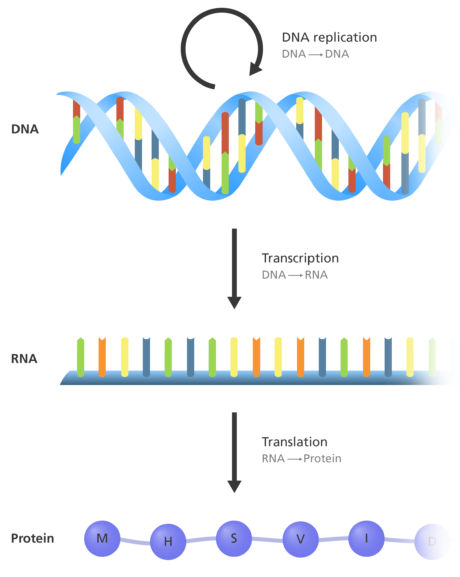
\includegraphics[width=0.5\textwidth]{figs/genome/central-dogma.png}}
  \caption[6pt]{The central dogma of molecular biology.}
  \label{fig:g-central-dogma-genome}
\end{figure}

At this stage, however, we should mention that biology is full of exceptions and surprises. The central dogma is a fundamental principle of molecular biology, but it is not the only way in which genetic information is used in living systems. For example, some RNA molecules possess catalytic activity, and some proteins bind to DNA to regulate gene expression. In addition, the central dogma does not account for the many ways in which genetic information can be modified, such as through mutations, recombination, or epigenetic changes. Nevertheless, the central dogma provides a useful framework for understanding how genetic information is stored, transmitted, and used in living systems.

In this chapter, we will begin to explore genomes and DNA sequences.
\marginnote{Even in stretches of DNA once thought to be “junk,” researchers have found recurring motifs and structural patterns — hints that randomness in the genome is often an illusion.}
Our goal is to investigate whether these sequences are simply random arrangements of nucleotides or if there are recognizable patterns that can be identified, even without considering genes. Understanding these patterns can provide valuable insights into the structure and function of DNA. We will focus on genes in the next chapter, where we will delve deeper into their roles and significance.

\section{Structure of Deoxyribonucleic Acid (DNA)}

Deoxyribonucleic acid (DNA) is a long molecule composed of nucleotides, which consist of a sugar called deoxyribose, a phosphate group, and a nitrogenous base~(Fig.~\ref{fig:g-dna-detail}). There are four types of nucleotides: cytosine (C), guanine (G), adenine (A), and thymine (T). DNA consists of two strands that twist around each other to form a double helix. The strands are held together by weak hydrogen bonds, with adenine pairing with thymine and cytosine pairing with guanine.

\begin{figure}
    \centering{
        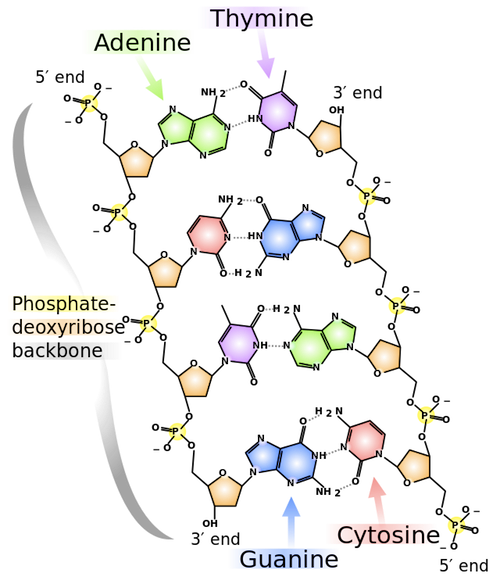
\includegraphics[width=0.6\textwidth]{figs/genome/dna-detail.png}
    }
    \caption[6pt]{The structure of DNA.}
    \label{fig:g-dna-detail}
  \end{figure}

  Each strand has a repeating pattern of deoxyribose sugars and phosphates, forming a strong sugar-phosphate backbone. The nucleotides are attached to this backbone, with one nucleotide connected to each sugar molecule.

Because the two strands are complementary, one strand can always be used to determine the sequence of the other. Both strands carry the same genetic information, which is crucial for accurate DNA replication.

The difference in bond strength gives DNA a zipper-like quality. The weak hydrogen bonds make it easy to unzip the strands, while the strong covalent bonds in the backbone protect the structure from damage. This design provides both flexibility and stability, allowing DNA to perform its role effectively in biological systems.

\section{Directionality of DNA Strands}

The two strands of DNA run in opposite directions, a property known as antiparallel orientation\marginnote{The antiparallel discovery was crucial for understanding DNA replication — it was one of the insights that helped Watson and Crick correctly model the double helix in 1953.}. To understand this concept, we need to examine the sugar group in the sugar-phosphate backbone. Chemists have established a system for numbering the carbon atoms in the sugar molecule, labeling them with ``prime'' notation, such as 1' (one-prime), 3' (three-prime), and so on. This notation helps organize the chemical structure and provides a clear reference for the orientation of the strands. Figure~\ref{fig:g-sugar} illustrates the atom numbering for the sugar group.

\begin{marginfigure}
  \centering{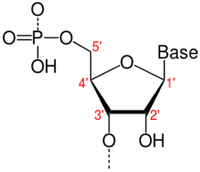
\includegraphics{figs/genome/sugar.png}}
  \caption[6pt]{Numbering of carbon atoms in a sugar group.}
  \label{fig:g-sugar}
\end{marginfigure}

In the DNA backbone, each sugar is linked to a phosphate group at its 5'-end (five-prime end) and to the next nucleotide through its 3'-end (three-prime end). The 5'-end of a DNA strand refers to the end with a free phosphate group attached to the 5' carbon of the sugar, while the 3'-end refers to the end with a free hydroxyl group (-OH) attached to the 3' carbon of the sugar.

This arrangement gives each DNA strand its own directionality. One strand runs from the 5' end to the 3' end, while the complementary strand runs in the opposite direction, from 3' to 5'. This antiparallel structure is critical for many biological processes, such as DNA replication and transcription. The enzymes involved in these processes recognize the direction of each strand and ensure that the genetic information is copied or read correctly.

The 5' to 3' orientation also plays an essential role in the regulation of gene expression, as this directionality influences how various molecules interact with DNA during cellular processes. Understanding this fundamental concept is crucial to grasping the mechanisms that underlie molecular biology and the flow of genetic information.

\section{Genome Size and Packaging}

The complete DNA sequence of an organism is called its genome. The genome represents the total genetic information contained within a cell, including the DNA in the nucleus and within any organelles. Interestingly, some organelles also contain their own DNA
\marginnote{Mitochondria and chloroplasts likely originated from ancient bacteria that formed symbiotic relationships with early eukaryotic cells—a concept known as the \textit{endosymbiotic theory}.}. In animals, this organelle is the mitochondrion, and in plants, it is the chloroplast. However, when we refer to the genome of a eukaryote, we usually mean the DNA in the nucleus. The genetic material in the mitochondria is referred to as the mitochondrial DNA (mtDNA) or mitochondrial genome.

In the nucleus, DNA is typically not a single continuous molecule but is instead divided into segments and organized into chromosomes. For example, humans have 23 pairs of chromosomes. However, we won't focus on chromosomes for now, so there's no need to worry about them in the next few lectures.

This structure allows the genome to be efficiently packaged and organized, facilitating processes such as cell division and gene expression. The size of the genome can vary greatly between species, but it always contains all the information necessary for the development, function, and reproduction of the organism.

So, what is the total length of the DNA sequence? It depends on the organism, as shown in Figure~\ref{fig:g-genome-size}. Prokaryotes, such as bacteria, have the shortest genomes. We measure DNA length in base pairs (bp), which refer to two nucleobases bound together by hydrogen bonds. Simply put, one base pair consists of one nucleotide on each strand of the DNA. The total number of nucleotides on one strand determines the overall size (or length) of the genome.

\begin{figure}
    \centering{
        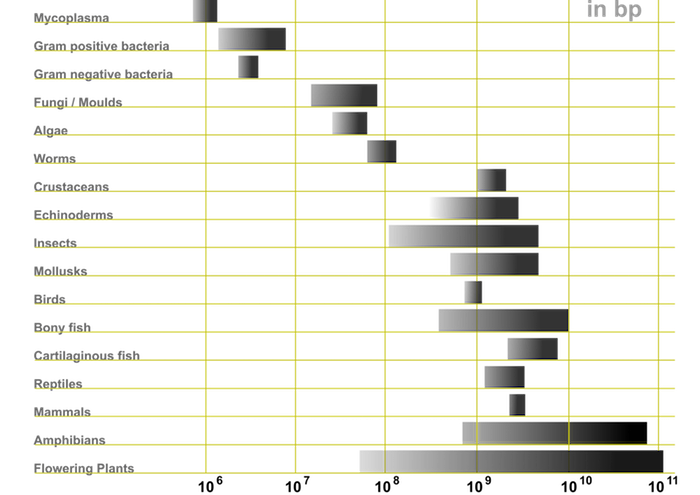
\includegraphics[width=0.95\textwidth]{figs/genome/genome-size.png}
    }
    \caption[6pt]{Genome sizes of various organisms.}
    \label{fig:g-genome-size}
  \end{figure}

Bacterial genomes typically range from 0.5 to 13 megabase pairs (Mbp), where one Mbp equals one million (10\textsuperscript{6}) base pairs. The abbreviation ``Mb'' is often used to represent megabases (megabase pairs). In prokaryotes, the genome is usually circular, while in eukaryotes it is typically linear and distributed among multiple chromosomes. This distinction has important implications for how DNA is replicated and organized within the cell.

Eukaryotic genomes are much larger\marginnote{Curiously, genome size does not correlate with organism complexity — an onion has far more DNA than a human. This puzzle is known as the \textit{C-value paradox}, reminding us that more DNA doesn’t necessarily mean a “more advanced” organism.}, ranging from 8 Mb to 670 gigabase pairs (Gb), with one Gb equaling one billion (10\textsuperscript{9}) base pairs. In contrast, viruses have much smaller genomes, ranging in size from 5 to 50 kilobase pairs (kb), where one kb equals one thousand (10\textsuperscript{3}) base pairs.

And what about us, humans? Our genome contains about 3,200 Mb (or 3.2 Gb). To put that in perspective, the first Harry Potter book, Harry Potter and the Philosopher’s Stone, contains approximately 76,944 words. With the average English word being just over five letters long, the book contains roughly 384,720 letters. If we represented each nucleotide in the human genome as a single letter, we would need the equivalent of about 8,300 copies of Philosopher’s Stone to write out the entire human genome. To visualize this further, a typical version of Harry Potter and the Philosopher’s Stone is about 2 cm thick. If we stacked 8,300 of these books, one on top of another, the stack would reach a height of around 166 meters.

If we could stretch out the DNA from a single human cell, it would form a very thin thread about 2 meters long. Despite this length, the DNA is tightly packed into the cell's nucleus, which is only about 5–10 micrometers in diameter. This incredible compaction is made possible because the DNA is wrapped around proteins called histones, forming a structure known as chromatin. This efficient organization allows the large amount of DNA to fit neatly inside the tiny space of the cell nucleus.

\section{Exploring Viral Genomes: Lambda Phage as a Case Study}

Let us start small—with a virus. The lambda phage\marginnote{The lambda phage has been a cornerstone of molecular biology since the 1950s—it helped scientists uncover how genes are regulated, leading to the discovery of genetic switches and laying groundwork for modern genetics.} is a bacterial virus that infects and destroys \textit{Escherichia coli} bacteria. This virus, like many others, has its genome fully sequenced and available for research. You may have noticed the scientific name \textit{Escherichia coli}. These names follow the rules of binomial nomenclature, a system that uses Latin names composed of a genus and species. For example, humans are classified as \textit{Homo sapiens}.

Now, back to the lambda phage. One of the sources for its genome information is GenBank\footnote{\url{https://www.ncbi.nlm.nih.gov/genbank}},
a sequence database maintained by the National Center for Biotechnology Information (NCBI). GenBank hosts a page dedicated to the lambda phage genome\footnote{\url{https://www.ncbi.nlm.nih.gov/nuccore/NC_001416.1}}.

The GenBank page
\marginnote{GenBank isn’t alone—similar databases include EMBL-EBI’s ENA in Europe and DDBJ in Japan. Together, these three form the International Nucleotide Sequence Database Collaboration, ensuring that every submitted sequence is synchronized and globally accessible.}
contains several key pieces of information.
It includes data about the scientists and research groups that sequenced and published the genome, as well as a detailed description of the genome’s structure. The page also lists the specific genes encoded within the genome and their functions. Finally, at the bottom of the page, you'll find the complete DNA sequence of the lambda phage, represented as a string of nucleotides (A, T, C, and G). This sequence is what we are most interested in for bioinformatics analyses. If you are curious about the meaning of the various fields and terms on GenBank's page, you can refer to the Sample GenBank Record page\footnote{\url{https://www.ncbi.nlm.nih.gov/genbank/samplerecord}}. Clicking on any of the terms will provide an explanation of their significance.

While all this information is available through the GenBank's web page, we are more focused on how to access it programmatically. This allows us to automate the retrieval of genomic data for further analysis and manipulation, which is essential for large-scale bioinformatics tasks. Programmatic access ensures reproducibility, scalability, and the ability to integrate data retrieval directly into analytical pipelines. 

In the following example, we will see how to retrieve the lambda phage genome sequence using Python:

\vspace*{3mm}
\begin{lstlisting}
>>> from Bio import Entrez, SeqIO
>>> Entrez.email = "blaz.zupan@fri.uni-lj.si"
>>> with Entrez.efetch(db="nucleotide", 
>>>   id="NC_001416", rettype="gb") as handle:
>>>    data = SeqIO.read(handle, "genbank")
>>> len(data.seq)
48502
>>> data.seq[:10]
Seq('GGGCGGCGAC')
\end{lstlisting}

The genome of {\em Lambda phage} contains 48,502 base pairs. We have the sequence for only one strand; the other strand is simply its reverse complement. The genome starts with three guanine nucleotides (G). Which nucleotide is the most abundant in the {\em Lambda phage} genome?

\vspace*{3mm}
\begin{lstlisting}
>>> from collections import Counter
>>> Counter(str(data.seq))
Counter({'G': 12820, 'A': 12334, 'T': 11986, 'C': 11362})
\end{lstlisting}

The most prevalent nucleotide in the {\em lambda phage} genome is guanine (G), followed by adenine (A), thymine (T), and cytosine (C). The genome is well balanced in terms of nucleotide frequency. The question now is whether this pattern holds true for all genomes. Since we have the necessary tools, we can test this with another organism.

Let's do this for the bacterium {\em Mycoplasma genitalium}, a tiny organism that causes sexually transmitted infections. It can lead to problems such as inflammation in the urinary tract (in men) or the cervix and pelvic area (in women). For bioinformatics, this bacterium is particularly interesting because it has one of the smallest genomes of all known free-living organisms.

\vspace*{3mm}
\begin{lstlisting}
>>> from Bio import Entrez, SeqIO
>>> Entrez.email = "blaz.zupan@fri.uni-lj.si"
>>> with Entrez.efetch(db="nucleotide", 
>>>   id="NC_000908.2", rettype="gb") as handle:
>>>    data = SeqIO.read(handle, "genbank")
>>> data.description
'NC_000908.2 Mycoplasma genitalium G37, complete sequence'
>>> len(data.seq)
580076
>>> Counter(data)
Counter({'A': 200544, 'T': 195711, 'G': 92306, 'C': 91515})
>>> n = sum(counts.values())
>>> for c in counts.keys():
>>>   print(f"{c}: {counts[c]:,} ({counts[c]/n:.1%})")
T: 195695 (33.7%)
A: 200543 (34.6%)
G: 92312 (15.9%)
C: 91524 (15.8%)
\end{lstlisting}

The genome of {\em M. genitalium} is not balanced. In fact, adenine (A) and thymine (T) are the most prevalent, and interestingly, their frequencies are almost equal. Similarly, the frequencies of cytosine (C) and guanine (G) are also nearly equal. This is a common feature of many genomes, where the adenine–thymine and cytosine–guanine pairs are balanced. This balance is important for the stability of the DNA double helix, as the adenine–thymine and cytosine–guanine pairs have different numbers of hydrogen bonds. Maintaining this balance helps preserve the stability of the DNA structure and has been evolutionarily selected to ensure the integrity of genetic information.

Of course, at this stage, we could test the prevalence and balance between A–T and C–G pairs in other organisms—for example, in humans. The smallest human chromosome is chromosome 21. Despite its small size, it plays a critical role in development and health. For instance, having an extra copy of chromosome 21 leads to Down syndrome. Fetching the sequence of this chromosome, even though it is relatively small, takes time, so it may help if we restructure our code to save the data locally for any subsequent rerun of the analysis.

\vspace*{3mm}
\begin{lstlisting}
  import os.path
  from Bio import Entrez, SeqIO
  from collections import Counter
  
  Entrez.email = "blaz.zupan@fri.uni-lj.si"
  
  organism_id = {
      "Hs_21": "NC_000021.9", # Homo sapiens genomic DNA
      "Pl": "NC_001416.1",  # Phage lambda
      "Mt": "AL123456.3",  # Mycobacterium tuberculosis
      "Mg": "NC_000908.2",  # Mycoplasma genitalium
      "Ec": "NC_000913",  # E coli
  }
  organism = "Hs_21"
  
  filename = f"data/{organism}.fasta"
  if os.path.exists(filename):
      print(f"Loading {organism} sequence from local file.")
      data = SeqIO.read(filename, "fasta")
  else:
      print(f"Fetching {organism} ...")
      with Entrez.efetch(
          db="nucleotide",
          id=organism_id[organism],
          rettype="gbwithparts",
          retmode="text"
      ) as handle:
          data = SeqIO.read(handle, format="genbank")
  
      print("Storing ...")
      with open("data/%s.fasta" % organism, "w") as f:
           SeqIO.write([data], f, "fasta")
  
  print(f"Genom eID: {data.id}")
  print(f"Description:\n{data.description}")
  print(f"Genome size: {len(data.seq):,}")
  
  counts = Counter(str(data.seq))
  n = sum(counts.values())
  for c in counts.keys():
      print(f"{c}: {counts[c]:,} ({counts[c]/n:.1%})")
\end{lstlisting}

The code above checks whether the sequence of the organism is already stored locally. If it is, it loads the sequence from the file; if not, it fetches the sequence from the NCBI database and stores it locally. This way, we can avoid repeatedly downloading the same data, which can be time-consuming and inefficient. When we run the code, we obtain the following result:

\vspace*{3mm}
\begin{lstlisting}
Loading Hs_21 sequence from local file.
Genom eID: NC_000021.9
Description: 
NC_000021.9 Homo sapiens chromosome 21, GRCh38.p14 Primary Assembly
Genome size: 46,709,983
N: 6,621,361 (14.2%)
G: 8,226,381 (17.6%)
A: 11,820,664 (25.3%)
T: 11,856,330 (25.4%)
C: 8,185,244 (17.5%)
M: 2 (0.0%)
R: 1 (0.0%)
\end{lstlisting}

Great — A–T and G–C pairs are balanced once more. But what about the other letters? In genome sequences, characters other than A (adenine), T (thymine), G (guanine), and C (cytosine) indicate ambiguous nucleotide bases or unique cases. These additional symbols follow the IUPAC (International Union of Pure and Applied Chemistry) nucleotide code:

\begin{itemize}
\item N: any nucleotide (A, T, G, or C), the specific base is unknown,
\item M: either A (Adenine) or C (Cytosine). M stands for ``amino'', because both adenine and cytosine have an amino group attached to their structures.
\item R: either A (Adenine) or G (Guanine). R stands for ``purine'', because both adenine and guanine are purines, which are a class of nitrogenous bases with a two-ring structure.
\end{itemize}

\section*{Accession Numbers}

You may notice that in the code so far we have used NCBI's accession numbers, that is, unique identifiers assigned to specific sequences in the National Center for Biotechnology Information (NCBI) databases. For example, the NC\_000021.9 accession number corresponds to Chromosome 21 of {\em Homo sapiens}, and AL123456.3 corresponds to the genome of {\em Mycobacterium tuberculosis}, the bacterium responsible for tuberculosis.

Accession numbers allow researchers to reference and access genome sequences, genes, or proteins easily. Typically, accession numbers are assigned when a new sequence is submitted to NCBI as part of a genome or protein record. To obtain them, researchers sequence the DNA, validate it, and submit the data through NCBI submission tools such as GenBank. To find an accession number, one can search for an organism, gene, or sequence of interest using NCBI’s search tools, such as Entrez, which will return the corresponding accession number for that specific dataset. For a start, one may also query any of the well-trained large language models to find the accession number for a specific organism or gene.

\section*{Time for Some Formalism}

To describe a nucleotide sequence, we will use lists of symbols from an alphabet $\mathcal{N} = {A, C, T, G}$. We will represent sequences as vectors and denote them with symbols such as $\vec{x}$, $\vec{s}$, and $\vec{t}$. Most often, we will be informal and omit the arrow, using symbols like $x$, $s$, and $t$ to represent sequences.

Consider now a nucleotide sequence $x$. This is a finite string over the alphabet $\mathcal{N}$, such that $x = x_1x_2x_3 \dots x_n$, where $x_i$ is an element of the string and $x_i \in \mathcal{N}$.

\section*{Multinomial Model of a Sequence}

The simplest (and least useful) model of a sequence is the multinomial model. This model simply specifies the probabilities with which each of the nucleotides appears in the sequence. The model assumes that nucleotides are independently and identically distributed. In statistics, this assumption is abbreviated as i.i.d., or independently identically distributed. ``Independently'' here means that the probability of encountering a symbol in a sequence does not depend on its position or on any neighboring symbols in the sequence. Intuition suggests that this may not be the case in DNA, but the multinomial model can still provide a foundation for reasoning about sequences—particularly for understanding how real DNA sequences deviate from the i.i.d. property.

The multinomial model of a DNA sequence is defined as $\vec{p} = (p_A, p_C, p_T, p_G)$, where $p_z = p(x_i = z)$ and $\sum_{z \in \{A, C, T, G\}} p_z = 1$.

Given a multinomial model, the probability of a sequence is
\[
P(x) = \prod_{i=1}^{n} p(x_i)
\]
Do you think this probability will be large, small, or perhaps extremely small? Why?

We have already estimated the parameters of the multinomial model in the code a few pages back, using relative frequencies for this task. Just to write it formally, the relative frequency of a nucleotide $z$ in a sequence $x$ is:
\[
\hat{p}_z = \frac{{\rm count}(z, x)}{n}
\]
where ${\rm count}(z, x)$ is the number of occurrences of nucleotide $z$ in the sequence $x$ and $n$ is the length of the sequence.

\section*{Finding Unusual DNA Words}

More than the probabilities of individual nucleotides, we might be interested in the probabilities of short subsequences of length $k$. Here, in this section, we will consider only dinucleotides, which are subsequences of length $k=2$. For example, we may want to observe whether a subsequence CG appears more often than would be expected by chance. Such short patterns, often referred to as "motifs," can reveal biologically meaningful features of the genome, such as regulatory elements or mutation hotspots.

By chance, using our multinomial model, the probability that a random nucleotide pair would form the combination C and G (i.e., the subsequence CG) is equal to $p_C \times p_G$. That’s straightforward. So what, then, is the probability of CG that we can estimate from the actual genome? We observe all the dinucleotides (there are $n - 1$ of them) and count how many are equal to CG. Thus, we estimate this probability as $\frac{N_{CG}}{n - 1}$, where $N_{CG}$ is the number of occurrences of the dinucleotide CG in the sequence $x$.

Next, we can compute the odds ratio, defined as the ratio between the observed probability of a dinucleotide and its expected probability under the multinomial model. An odds ratio of 1 indicates the dinucleotide occurs as often as expected, while values above or below 1 indicate overrepresentation or underrepresentation, respectively. The expected probability is calculated under the i.i.d. assumption, meaning that the genome sequence is treated as if there is no dependency or order between nucleotides:
\[
{\rm odds ratio} = \frac{N_{CG}/(n-1)}{p_C \times p_G}
\]

Often, instead of the odds ratio, we report the log-odds ratio, as it provides a symmetrical measure of deviation centered at 0. Subsequences that occur more frequently than expected have positive log-odds ratios, while those that occur less frequently have negative values. This transformation also makes it easier to compare results across different sequences, since ratios that differ by orders of magnitude are brought to a more manageable numerical scale.

Time to implement this in code. We start with the generator of dinucleotides:

\vspace*{3mm}
\begin{lstlisting}
def tuple_walk(s, k=2):
  """Generate all k-tuples from sequence s."""
  for i in range(len(s) - (k-1)):
    yield s[i:i+k]

def count_tuple(s, w):
  """Count words w in sequence s."""
  return sum(1 for ss in tuple_walk(s, len(w)) if ss == w)
\end{lstlisting}

Let's use these functions on a short sequence, just to check it out:

\vspace*{3mm}
\begin{lstlisting}
>>> s = "ACCTAGGCT"
>>> list(tuple_walk(s))
['AC', 'CC', 'CT', 'TA', 'AG', 'GG', 'GC', 'CT']
>>> count_tuple(s, "CT")
2
\end{lstlisting}

Fine. This seems to work. Now we can implement the odds ratio computation, and put all the code together to analyze the H. sapiens chromosome 21:

\vspace*{3mm}
\begin{lstlisting}
from Bio import SeqIO
from collections import Counter
import math

def tuple_walk(s, k=2):
    """Generate subsequences of length k."""
    for i in range(len(s)-1):
        yield s[i:i+k]

def count_tuple(s, w):
    """Count words w in sequence s."""
    return sum(1 for ss in tuple_walk(s, len(w)) if ss == w)

organism = "Hs_21"

filename = f"data/{organism}.fasta"
s = str(SeqIO.read(filename, "fasta").seq)

subsequence = "CG"
count = count_tuple(s, subsequence)
print(f"Count of {subsequence} on original sequence: {count:,}")

n = len(s)
p_nucleotide = {k: v/n for k, v in Counter(s).items()}
p = math.prod(p_nucleotide[x] for x in subsequence)
print(f"Expected: {int((p * n)):,}")
odds = (count / n) / p
print(f"Odds ratio: {odds:.2f}")
print(f"Log odds ratio: {math.log(odds):.2f}")
\end{lstlisting}

Running the code we get:

\vspace*{3mm}
\begin{lstlisting}
Count of CG on original sequence: 462,299
Expected: 1,441,553
Odds ratio: 0.32
Log odds ratio: -1.14
\end{lstlisting}

The dinucleotide \textbf{CG} appears less frequently than expected by chance. The log-odds ratio is negative, indicating that the observed frequency of \textbf{CG} is lower than the expected frequency under the multinomial model. This result is not surprising, as the dinucleotide \textbf{CG} is known to be underrepresented in the human genome. However, \textbf{CG} dinucleotides are often concentrated in specific regions called \textbf{CpG islands}, which are associated with gene regulation, DNA methylation, and other epigenetic modifications.

In the abbreviation ``CpG,'' the \textbf{p} refers to the phosphate group that links the cytosine (C) and guanine (G) nucleotides in the DNA backbone. \textbf{CpG islands} are typically located near gene promoters and play a crucial role in regulating gene expression (as we will discuss in later chapters).

\begin{marginfigure}
  \centering{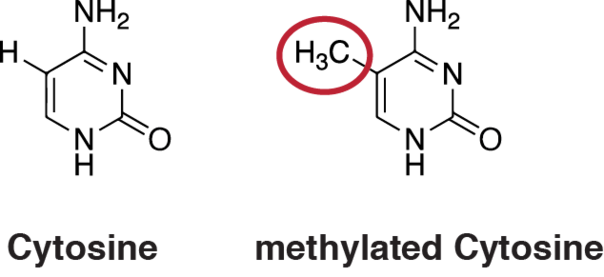
\includegraphics{figs/genome/dna-methylation.png}}
  \caption[6pt]{DNA methylation.}
  \label{fig:g-dna-methylation}
\end{marginfigure}

The lower frequency of \textbf{CG} dinucleotides in the genome is primarily due to the methylation of cytosine, which converts it into 5-methylcytosine. This modification plays a key role in gene silencing and epigenetic regulation. Over evolutionary time, methylated cytosines tend to mutate into thymines (T) through a process called deamination. This mutation leads to a gradual loss of \textbf{CG} dinucleotides from the genome, resulting in fewer \textbf{CpG islands} than would be expected by chance.

This reduction in \textbf{CG} content may have provided evolutionary benefits\marginnote{The discovery of DNA methylation in the 1940s by Rollin Hotchkiss gave rise to the field of epigenetics, which studies changes in gene expression without altering the DNA sequence. These changes, such as the methylation of cytosine in CpG dinucleotides, can silence or reduce gene activity. Importantly, epigenetic modifications can be inherited during cell division and, in some cases, passed from one generation to the next, meaning that environmental factors can influence not only an individual’s gene expression but also potentially affect their offspring.}. Methylation and the resulting mutations likely played a role in genome defense mechanisms, such as \textit{silencing transposable elements} (DNA sequences that can move within the genome) to prevent them from disrupting functional genes. Additionally, selective pressure may have favored a reduced number of CpG dinucleotides outside CpG islands, minimizing unnecessary mutations that could interfere with essential gene regulation processes.

Just one more note about methylation: the mechanism that retains methylation during DNA replication is called maintenance methylation. This process is carried out by an enzyme called DNA methyltransferase 1 (DNMT1). When DNA is replicated, the new strand is synthesized without methylation marks. DNMT1 recognizes hemimethylated DNA (where the parent strand is methylated and the newly synthesized strand is not) and adds methyl groups to the corresponding sites on the new strand. This ensures that the methylation pattern is preserved across cell divisions, thereby maintaining the epigenetic state and regulatory memory of the genome.

Other than CpG, the dinucleotides TpA and CpA are also of interest in genomic studies, each for different reasons:

\begin{itemize}
    \item TpA: This dinucleotide is often underrepresented in genomic sequences, likely due to its association with instability in the DNA double helix. TA pairs form only two hydrogen bonds, making them more prone to mutations and breakage. This dinucleotide also plays a role in certain regulatory regions like promoters and is found in repetitive elements.
    
    \item CpA: CA dinucleotides are frequently found in regions of active gene expression and are often involved in alternative splicing. Methylation of CpA is also emerging as a topic of interest, particularly in non-CpG methylation, which is being linked to developmental and tissue-specific gene regulation.
\end{itemize}

Both of these dinucleotides, along with others, contribute to the broader understanding of DNA sequence evolution, mutability, and regulation of gene expression.

\section{Where to Go from Here}

This chapter offers just a glimpse into the world of genomes and DNA sequences. In the next chapter, we will continue our exploration by focusing on how genes are identified within these sequences and how computational methods can help characterize their structure and function.

\section*{Ideas for Mini Projects}

For simplicity, in all the exercises below, all analyses may be performed using only one strand of the DNA sequence (as provided in the genome file), without considering the reverse complement. Notice that this strand is also referred to as plus strand.

\begin{enumerate}
\item Consider two groups of bacteria: 
\begin{itemize}
\item Group A, free-living and metabolically active: \textit{Mycobacterium tuberculosis} (NCBI accession id \texttt{AL123456.3}), \textit{Pseudomonas aeruginosa} (\texttt{NC\_002516.2}), \textit{Streptomyces coelicolor} (\texttt{NC\_003888.3}),
\item Group B, parasitic or symbiotic: \textit{Mycoplasma genitalium} (\texttt{NC\_000908.2}), \textit{Chlamydia trachomatis} (\texttt{NC\_000117.1}), \textit{Borrelia burgdorferi} (\texttt{NC\_001318.1}), \textit{Helicobacter pylori} (\texttt{NC\_018939.1}).
\end{itemize}
With these two groups, perform the following tasks:
\begin{enumerate}
\item Find out what organisms in Group A have in common, and what organisms in Group B have in common (you may use any chatbot or online resource).
\item Write Python code (using Biopython's Entrez/SeqIO or similar) that loads the genome sequences of these organisms and compares their genome lengths. What differences do you observe?
\item Extend the code to compute the frequency of codons (triplets of nucleotides) for each genome. Do you notice any systematic differences between Group A and Group B?
\item Finally, use biological reasoning (with the help of a chatbot or literature if needed) to explain \textit{why} these differences in genome size and codon usage might exist between the two groups.
\end{enumerate}

\item Fetch the genome sequences of the three shortest non-Y human chromosomes and analyze their nucleotide composition. Compare the frequencies of A/T versus C/G across each chromosome. Do you observe a consistent difference? If so, determine whether this pattern has an evolutionary explanation using AI chatbots or external references.

\item For the genome sequences from the previous exercise (shortest non-Y human chromosomes), compute the frequency of CpG dinucleotides, and their odds ratio (observed vs. expected). Do you observe any interesting pattern? Can you explain it?

\item A plausable hypothesis is that the CpG depletion in the human genome is directly caused by DNA methylation of cytosines in CpG dinucleotides, followed by mutation (C to T), which gradually removes CpG sites over evolutionary time. If this is the case, then this effect should not be present in organisms with no DNA methylation. Examples of such organisms are budding yeast \textit{Saccharomyces cerevisiae} (consider, for instance, chromose I, \texttt{NC\_001216.2}), bacteria \textit{Escherichia coli} (\texttt{NC\_000913}) and nematode \textit{Caenorhabditis elegans} (chromosome I,\texttt{NC\_003370.1}), which has a very low genome methylation rate. Fetch their genomes and analyze if the absence of DNA methylation is reflected in the frequency of CpG dinucleotides. Always compare the observed frequency of CpG dinucleotides with the expected frequency under the multinomial model.

\item Conside the genome of \textit{Escherichia coli} \texttt{NC\_000913}, and compare the observed and expected frequencies of motives \texttt{AAAAA} and \texttt{GGGGG}. Do these motives occur more or less frequently than expected? Was this expected and if so, why? Use AI chatbots or external references to explain the differences.

\item Consider the motif \texttt{GATCC} in the \textit{Escherichia coli} genome. Considering only the plus strand, the observed frequency of this motif is 0.00090, while its expected frequency under the multinomial (independent nucleotide) model is 0.00099 – only slightly higher. In other words, although this motif appears somewhat less often than expected, the difference does not immediately look significant. Investigate this by performing a permutation (randomization) test. Generate, say, 1000 randomized sequences with the same genome length and nucleotide composition, count how often this motif appears in each, and record the propotion of sequences where the count is less than or equal to the observed count. This is the p-value for our test, that is, the probability of observing a count as low as or lower than the observed count in a random sequence.
\end{enumerate}



